\pc{3}{11/11}

\question Suppose a process in Host $V$ has a UDP socket with port number 6789. 
Suppose both Host $A$ and Host $B$ each send a UDP segment to Host $C$ with destination port number 6789.
Will both of these segments be directed to the same socket at Host $C$?
If so, how will the process at Host $C$ know that these two segments originated from two different hosts?

\question In our RDT protocols, why did we need to introduce timers?

\question Consider Figure \ref{fig:prac-3-1}.
What are the source and destination port values in the segment flowing from the server back to the clients' processes?
What are the IP addresses in the network-layer datagrams carrying the transport-layer segments?

\begin{figure}
    \centering
    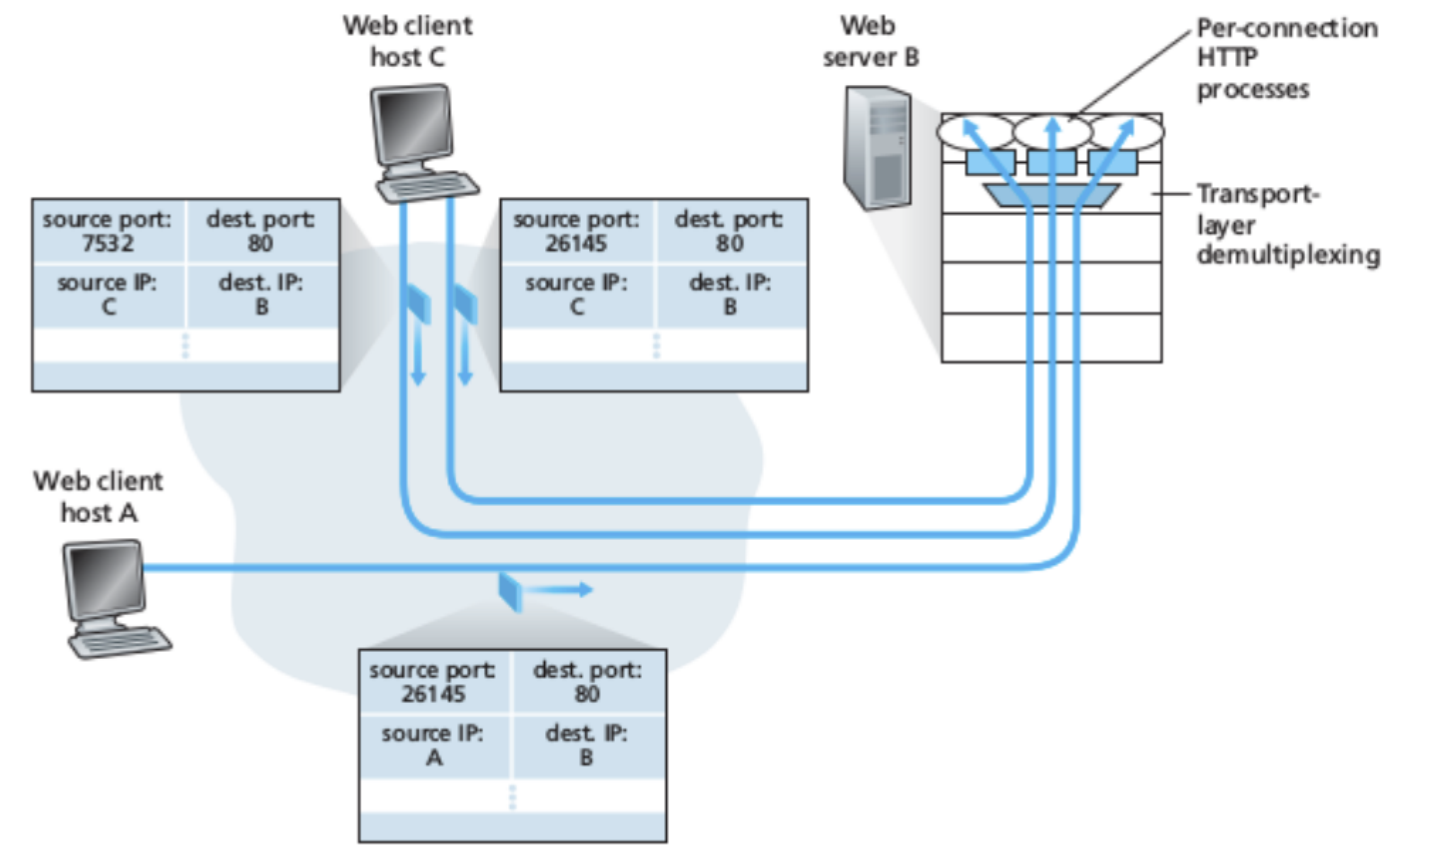
\includegraphics[width=0.6\textwidth]{images/prac-3-1.png}
    \caption{}
    \label{fig:prac-3-1}
\end{figure}

\question Suppose an application uses RDT 3.0 as its transport layer porotocol. As the stop-and-wait protocol has very low channel utilisation, the designers of this application let the receiver keep sending back a number (more than two) of alternating ACK 0 and ACK 1 even if the corresponding data have not arrived at the receiver.
Would this application design increase the channel utilisation? Why?
Are there any potential problems with this approach? Explain.

\question Consider the GBN and SR protocols.
Suppose the sequence number space is of size $k$.
What is the largest allowable sender window that will avoid the occurrence of problems such as that in Figure \ref{fig:prac-3-2} for each of these protocols?

\begin{figure}
    \centering
    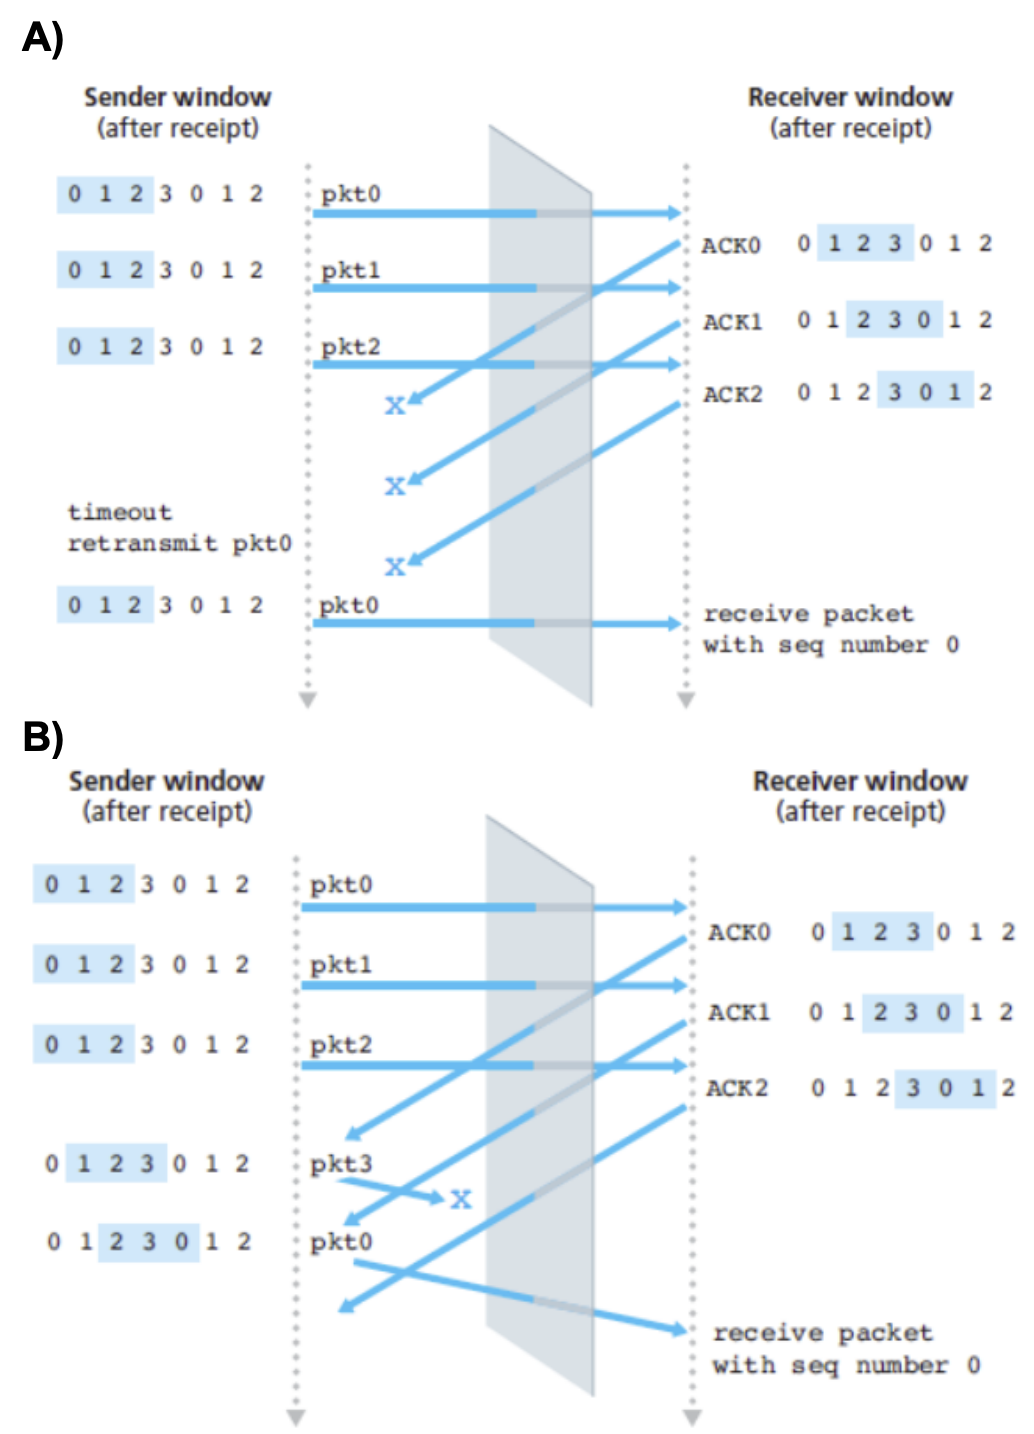
\includegraphics[width=0.5\linewidth]{images/prac-3-2.png}
    \caption{}
    \label{fig:prac-3-2}
\end{figure}
